\documentclass[10pt,letterpaper]{article}

\usepackage[letterpaper,hmargin=0.7in,vmargin=0.95in]{geometry}
\usepackage{enumitem,xurl,hyperref,graphicx}

\hypersetup{
  pdfauthor={Sangwon Kim},
  pdftitle={Curriculum Vitae - Sangwon Kim},
  pdfsubject={Curriculum Vitae},
  pdfkeywords={Sangwon Kim, curriculum vitae, Quasiclassical Tunneling Theory, Quantum Optics}
}

\setlength{\parindent}{0pt}

\newlength{\entrywidth}
\newlength{\itemwidth}
\settowidth{\itemwidth}{159.\enspace}

\newcommand{\entry}[2]{%
  \par\begingroup\noindent\hangindent=\entrywidth
  \makebox[\entrywidth][l]{#1}#2\par\endgroup\addvspace{\medskipamount}}

\newcommand{\cvitem}[2]{%
  \par\begingroup\noindent\hangindent=\itemwidth
  \makebox[\itemwidth][r]{#1.\enspace}#2\par\endgroup\addvspace{\medskipamount}}

\begin{document}

\begin{center}
  {\Large\bfseries Curriculum Vitae\par}
  \bigskip
  (Updated on Aug 20, 2026)
\end{center}
\bigskip

\hrulefill

\begin{minipage}[t]{0.75\linewidth}
  \section*{Sangwon Kim}
  \vspace{0pt}
  \begin{tabular}{@{}c@{\enspace}l@{}c@{\enspace}l@{}}
    $\cdot$ & Address  & : & Department of Physics, KAIST\\
            &          &   & 291 Daehak-ro, Yuseong-gu\\
            &          &   & Daejeon 34141, Republic of Korea\\
    $\cdot$ & Office   & : & Room 211, Building E6-6\\
    $\cdot$ & Phone    & : & +82-10-9990-1357\\
    $\cdot$ & Email    & : & \href{mailto:s4ngw0n@kaist.ac.kr}{\texttt{s4ngw0n@kaist.ac.kr}}\\
    $\cdot$ & Homepage & : & \url{https://s4ngw0n.github.io/}
\end{tabular}
\end{minipage}\hfill
\begin{minipage}[t]{0.2\linewidth}
  \vspace{0pt}
  \raggedleft
  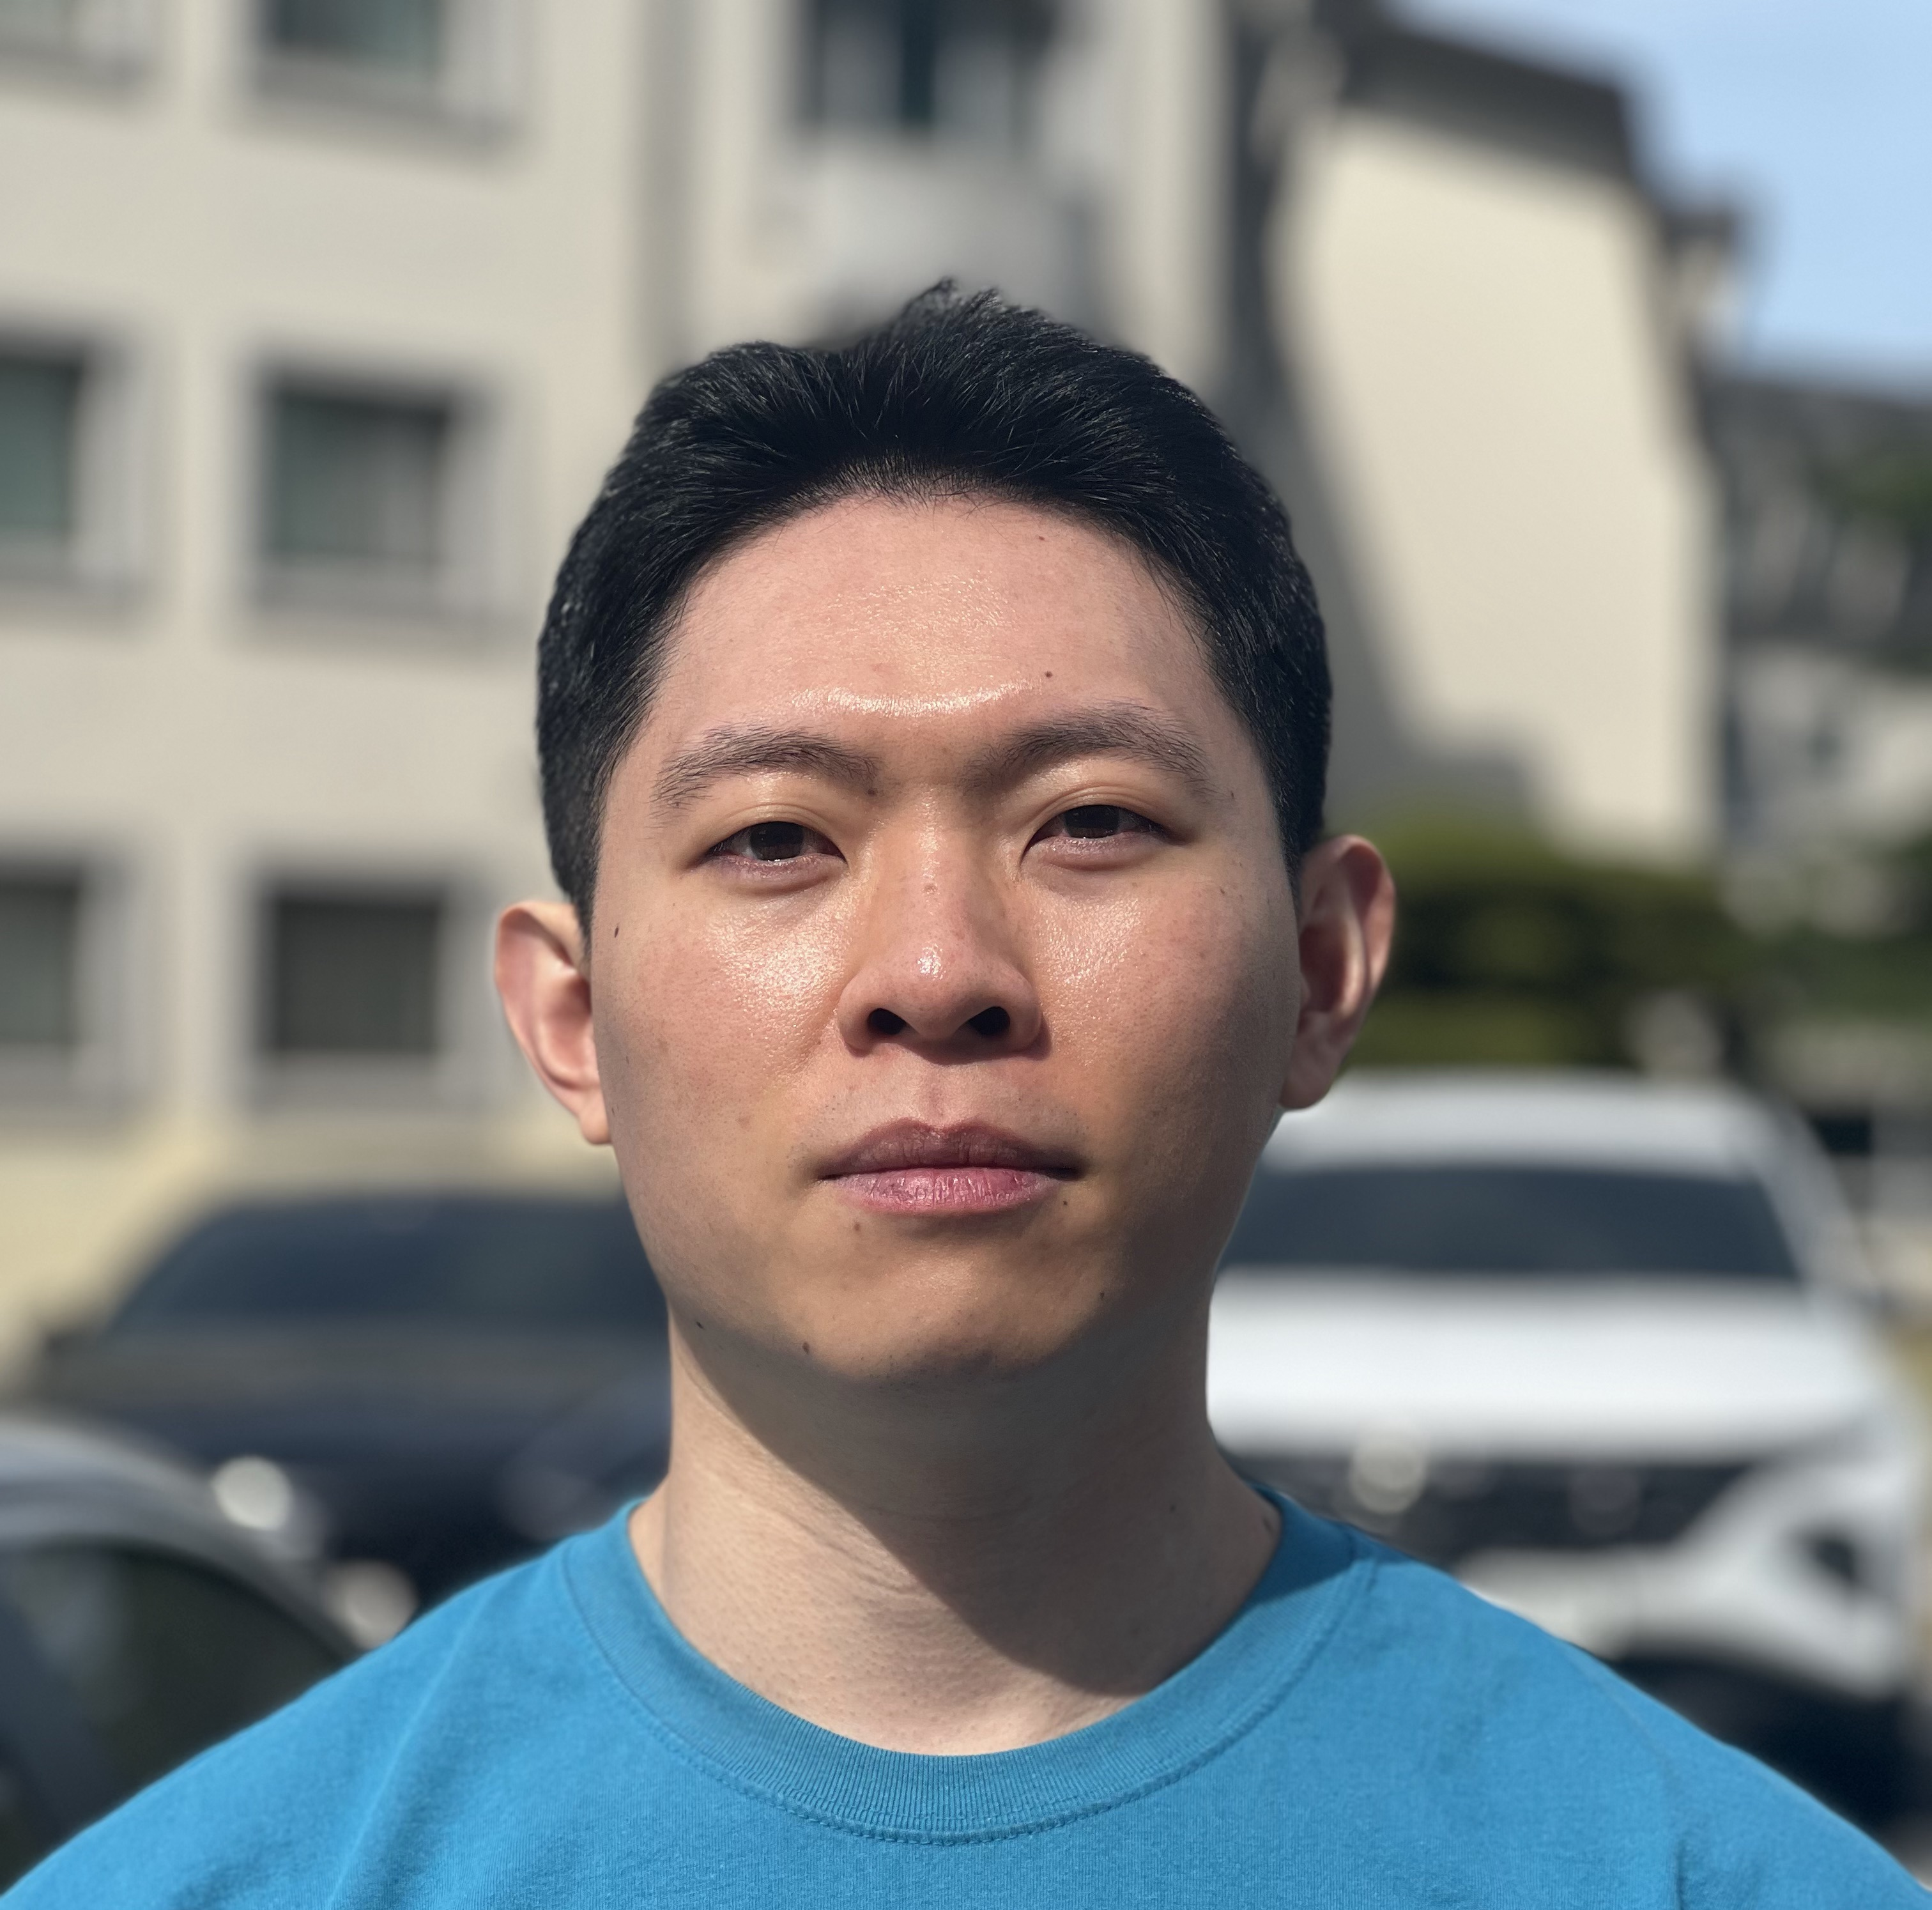
\includegraphics[
    width=\linewidth,
    height=7\baselineskip,
    keepaspectratio
  ]{photo.jpeg}
\end{minipage}\hspace*{1em}

\hrulefill

\section*{Research Interests}
$\cdot$ Ultrafast tunneling in nanocontacts\\
$\cdot$ Quasiclassical quantum theory\\
$\cdot$ Bohmian mechanics\\
$\cdot$ Quantum optics\\

\section*{Education}
\settowidth{\entrywidth}{0000/00/00 - 0000/00/00\quad\enspace}

\entry{2019/02/25 - 2026/08/21}{(Scheduled) Ph.D.\ in Physics, Korea Advanced Institute of Science and Technology, Korea\\
  (Thesis: Quasiclassical theory of nonadiabatic tunneling in nanocontacts driven by \\classical and quantum light)}
\entry{2014/03/01 - 2019/02/24}{B.S.\ in Physics, Korea Advanced Institute of Science and Technology, Korea}

\section*{Awards/Appreciation}
\settowidth{\entrywidth}{Dec 2025\qquad}

\entry{May 2024}{Best Student Paper Award\\
  \quad ALTA 2024}

\section*{Publication List}
\cvitem{3}{(Submitted) Electronic Switching at the Atomic Spatio-Temporal Scale\\
Marwin Gedamke, Sebastian Grossenbach, Sven Väth, Matthias Falk, Stefan Eggert, \textbf{Sangwon Kim}, Andrey S. Moskalenko, Daniele Brida, Markus Ludwig, and Alfred Leitenstorfer}
\cvitem{2}{(Submitted) Tunneling driven by quantum light described via field Bohmian trajectories\\
\textbf{Sangwon Kim}, Seongjin Ahn, Denis V. Seletskiy, and Andrey S. Moskalenko\\
\href{https://doi.org/10.48550/arXiv.2507.15972}{arXiv:quant-ph/2507.15972}}
\cvitem{1}{Quasiclassical theory of non-adiabatic tunneling in nanocontacts induced by phase-controlled ultrashort light pulses\\
\textbf{Sangwon Kim}, Tobias Schmude, Guido Burkard, and Andrey S. Moskalenko\\
\href{https://doi.org/10.1088/1367-2630/ac1552}{New. J. Phys. 23 083006 (2021)}. [\href{https://doi.org/10.48550/arXiv.2011.15125}{arXiv:cond-mat.mes-hall/2011.15125}]}

\section*{Oral Presentations}
\cvitem{2}{QAMTS 2024 at Donostia-San Sebastián, Spain (June 2024)\\
Quasiclassical approach to dynamical aspects of tunneling
in nanocontacts induced by ultrashort light pulses}
\cvitem{1}{OPC 2021 at Jeju, Korea (Jul. 2021)\\
Quasiclassical theory of non-adiabatic tunneling in
nanocontacts induced by ultrashort light pulses}

\section*{Conferences Participated (Poster Presentation)}
\cvitem{9}{UP 2026\\ Sapporo, Japan (August 2 - 7, 2026)}
\cvitem{8}{ALTA 2026\\ Jeju, Korea (May 6 - 9, 2026)}
\cvitem{7}{QAMTS 2024\\ Donostia-San Sebastián (Basque Country), Spain (June 16 - 21, 2024)}
\cvitem{6}{ALTA 2024\\ Jeju, Korea (May 1 - 4, 2024)}
\cvitem{5}{GRC Ultrafast Phenomena in Cooperative Systems\\ Lucca (Barga), Italy (February 4 - 9, 2024)}
\cvitem{4}{ALTA 2023\\ Jeju, Korea (May 1 - 4, 2003)}
\cvitem{3}{ICAMD 2021\\ Jeju, Korea (December 6 - 10, 2021)}
\cvitem{2}{OPC 2021\\ Jeju, Korea (July 4 - 7, 2021)}
\cvitem{1}{GRS/GRC Ultrafast Phenomena in Cooperative Systems\\ Lucca (Barga), Italy (February 1 - 7, 2020)}

\section*{Teachings}
\cvitem{14}{Spring 2026, Quantum Optics (PH624), TA, KAIST}
\cvitem{13}{Fall 2025, General Physics I (PH141), Vice Head TA, KAIST}
\cvitem{12}{Spring 2025, General Physics II (PH142), TA, KAIST}
\cvitem{11}{Fall 2024, General Physics II (PH142), TA, KAIST}
\cvitem{10}{Fall 2023, Graduate Quantum Mechanics II (PH504), TA, KAIST}
\cvitem{9}{Spring 2023, Graduate Classical Mechanics (PH505), TA, KAIST}
\cvitem{8}{Fall 2022, Physics Experiment I (PH251), TA, KAIST}
\cvitem{7}{Spring 2022, Quantum Optics (PH624), TA, KAIST}
\cvitem{6}{Fall 2021, Nonlinear Optics (PH721), TA, KAIST}
\cvitem{5}{Spring 2021, Graduate Classical Mechanics (PH505), TA, KAIST}
\cvitem{4}{Fall 2020, Classical Mechanics II (PH222), TA, KAIST}
\cvitem{3}{Spring 2020, Classical Mechanics I (PH221), TA, KAIST}
\cvitem{2}{Fall 2019, Experiment Oriented General Physics II (PH172), TA, KAIST}
\cvitem{1}{Spring 2019, General Physics II (PH142), TA, KAIST}

\section*{Other Activities}
\cvitem{2}{Visited femtoQ, Prof. Denis V. Seletskiy Group, Polytechnique Montréal\\
Montréal, Canada (December 5 - December 20, 2025).}
\cvitem{1}{Visited Prof. Guido Burkard Group and Prof. Alfred Leitenstorfer Group, Universität Konstanz\\
Konstanz, Germany(January 7 - February 17, 2020).}

\section*{Skills}
\cvitem{1}{Professional working proficiency in English.}
\cvitem{2}{Proficient in Mathematica, Maple, and Python/Jupyter.}
\cvitem{3}{Experienced with Linux Bash and C.}
\cvitem{4}{Completed all coursework required for a Bachelor's degree in Electrical Engineering, although the degree was not formally awarded.}
\cvitem{5}{Fully audited (participated all course activies including homeworks and exams) the following courses:\\
$\cdot$ Modern Algebra I (MAS311)}

\end{document}
